\documentclass[11pt,a4paper]{article}
\usepackage[dvipsnames]{xcolor}
\usepackage[utf8]{inputenc}
\usepackage{amsmath}
\usepackage{mathtools}
\usepackage{marvosym}
\usepackage{wrapfig}
\usepackage{hyperref}
\usepackage{float}
\usepackage{multicol}
\hypersetup{colorlinks,citecolor=black,filecolor=black,linkcolor=black,urlcolor=black}
\usepackage{pdfpages}
\usepackage{amsfonts}
\usepackage{amssymb}
\usepackage{fancyhdr}
\usepackage{chemfig}
\usepackage{graphicx}
\usepackage{t1enc}
\usepackage[magyar]{babel}
\usepackage{bm}
\usepackage{tikz, tcolorbox}
\usepackage{verbatim}
\usepackage{amsmath,esint}
\usepackage{setspace}
\usepackage{qtree}
\usepackage{multido}
\newcommand{\Pointilles}[1]{%
\par\nobreak
\noindent\rule{0pt}{1.5\baselineskip}% Provides a larger gap between the preceding paragraph and the dots
\multido{}{#1}{\noindent\makebox[\linewidth]{\dotfill}\endgraf}
\bigskip% Gap between dots and next paragraph
}
\usepackage{pgfplots}
\pgfplotsset{height = 10cm, width=15cm,compat=1.9}
\usepackage[left=2cm,right=2cm,top=2cm,bottom=2cm]{geometry}
\setlength{\parindent}{0pt}
\setlength{\parskip}{0em}
\pagestyle{fancy}
\fancyhf{}
\cfoot{\thepage. oldal}
\begin{document}

\begin{titlepage}
\centering


\includegraphics[width=.8\textwidth]{bme_logo_nagy.jpg}

\vspace{1em}

{
\large
BUDAPESTI MŰSZAKI ÉS GAZDASÁGTUDOMÁNYI EGYETEM GÉPÉSZMÉRNÖKI KAR
}

\vspace{8em}

{
\Huge
\textbf{CÍM}
}

\vspace{8em}

{
\huge
Görbék, felületek és transzformációk geometriája mérnököknek

\vspace{.2em}

\large
(BMETE94AX11)
}

\vspace{4em}

{
\Large
\textit{Készítette:}\\
\vspace{.5em}
\textbf{Név 2, Név 2 }
}
\vspace{4em}
%------------------------------------------------------------------------------------------
%------------------------------------------------------------------------------------------
%------------------------------------------------------------------------------------------
%Itt ennél a résznél mi tikz picture használtunk, hogy éles vector grafikus képeket kapjunk, viszont a az alábbi kommentelt kóddal tudtok beilleszteni képet akár .png vagy .pdf formátumban. Fontos, a kép legyen a mappában.

%\begin{center}
%    \fbox{\includegraphics[scale = 0.3]{1.png}}
%\end{center}

%------------------------------------------------------------------------------------------
%------------------------------------------------------------------------------------------
%------------------------------------------------------------------------------------------


\begin{center}
    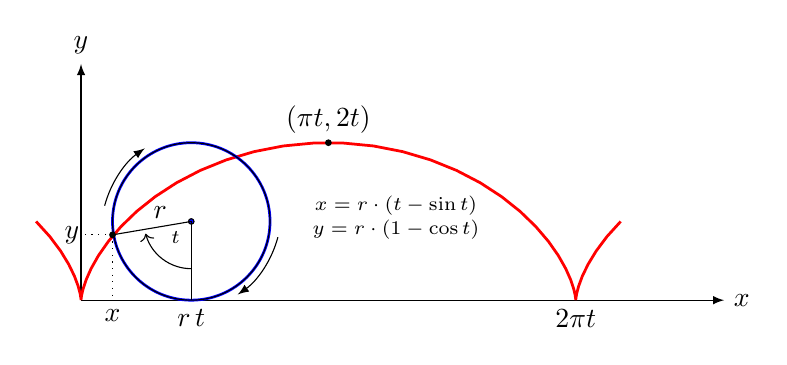
\begin{tikzpicture}
    \coordinate (O) at (0,0);
    \coordinate (A) at (0,3);
    \def\r{1} % radius
    \def\c{1.4} % center
    \coordinate (C) at (\c, \r);
  
  
    \draw[-latex] (O) -- (A) node[anchor=south] {$y$};
    \draw[-latex] (O) -- (2.6*pi,0) node[anchor=west] {$x$};
    \draw[red,domain=-0.5*pi:2.5*pi,samples=50, line width=1] 
         plot ({\x - sin(\x r)},{1 - cos(\x r)});
    \draw[blue, line width=1] (C) circle (\r);
    \draw[] (C) circle (\r);
  
    % coordinate x 
    \def\x{0.4} % coordinate x
    \def\y{0.83} % coordinate y
    \def\xa{0.3} % coordinate x for arc left
    \def\ya{1.2} % coordinate y for arc left
    \coordinate (X) at (\x, 0 );
    \coordinate (Y) at (0, \y );
    \coordinate (XY) at (\x, \y );
  
    \node[anchor=north] at (X) {$x$} ;
  
    % draw center of circle
    \draw[fill=blue] (C) circle (1pt);
  
    % draw radius of the circle
    \draw[] (C) -- node[anchor=south] {\; $r$} (XY);
  
    % bottom of circle, radius to the bottom
    \coordinate (B) at (\c, 0);
    \draw[] (C) -- (B) node[anchor=north] {$r \, t$};
  
    % projections of point XY
    \draw[dotted] (XY) -- (X);
    \draw[dotted] (XY) -- (Y) node[anchor=east, xshift=1mm] {$\quad y$};
  
    % arc theta
    % start arc
    \coordinate (S) at (\c, 0.4);
    \draw[->] (S) arc (-90:-165:0.6);
    \node[xshift=-2mm, yshift=-2mm] at (C) {\scriptsize $t$};
  
    % arc above
    \coordinate (AA) at (\xa, \ya);
    \draw[-latex, rotate=25] (AA) arc (-220:-260:1.3);
  
    % arc below
    \def\xb{2.5} % coordinate x for arc bottom
    \def\yb{0.8} % coordinate y for arc bottom
    \coordinate (AB) at (\xb, \yb);
    \draw[-latex, rotate=-10] (AB) arc (-5:-45:1.3);
  
  
  
    % XY dot
    \draw[fill=black] (XY) circle (1pt);
  
  
    % top label
    \coordinate (T) at (pi, 2);
    \node[anchor=south] at (T)  {$(\pi t, 2 t )$} ;
    \draw[fill=black] (T) circle (1pt);
  
    % equations
    \coordinate (E) at ( 4,1.2);
    \coordinate (F) at ( 4,0.9);
    \node[] at (E) {\scriptsize $x=r \cdot (t - \sin t)$};
    \node[] at (F) {\scriptsize $y=r\cdot (1 - \cos t)$};
  
    % label 2pi a
    \coordinate (TPA) at (2*pi, 0);
    \node[anchor=north] at (TPA) {$2 \pi t$};
  
  
    \end{tikzpicture}
  \end{center}
  \vspace{4em}
{
\large
BUDAPEST, 2023
}
\end{titlepage}

\setstretch{1.1}
{\Large \textbf{Bevezetés:} \par}
A ciklois egy lenyűgöző matematikai görbe, amely már évszázadok óta izgatja a matematikusokat és tudósokat. Ebben a részletes áttekintésben felfedezzük a ciklois görbe tulajdonságait, történetét és alkalmazásait.
\\
{\Large \textbf{Definíció és parametrikus egyenletek:}\par}
A ciklois egy görbe, amelyet egy pont rajzol le egy kerek kerék peremén, ahogy az egyenes vonal mentén gurul. A parametrikus egyenletei Descartes koordinátákban:
$$x(t) = r \cdot (t - \sin(t))$$
$$y(t) = r \cdot (1 - \cos(t))$$
Ahol:
\begin{itemize}
    \setlength\itemsep{3pt}
    \item \(x\) és \(y\) a ciklois egy pontjának koordinátái.
    \item \(r\) a gördülő kör sugarát jelöli.
    \item \(t\) a paraméter, amely változik, ahogy a pont mozog a görbén.
\end{itemize}

{\Large \textbf{Történelmi jelentőség:}\par}

A cikloisnak gazdag történelme van, amely a 17. századig nyúlik vissza, amikor először Mersenne, Roberval és Galilei tanulmányozták a görbét. Evangelista Torricelli és Christiaan Hoygens jelentős hozzájárulásokat tettek a görbe megértéséhez. Huygens például a cikloist használta egy pontosabb ingaóra tervezéséhez.\\

{\Large\textbf{Tulajdonságok:}\par}
A ciklois számos érdekes tulajdonsággal rendelkezik: Zárt görbe, ami azt jelenti, hogy visszatér a kiindulási pontra egy periódus után. Egy ciklois egyik ívjének hossza 8-szorosa a gördülő kör sugarának. A ciklois a legrövidebb idő alatt lezáródó görbe, ami azt jelenti, hogy egy rajta lecsúszó részecske a gravitáció hatására a legrövidebb idő alatt éri el a végpont más úthoz képest.\\

{\Large\textbf{Alkalmazások:}\par}
\begin{itemize}
    \item \textbf{Mérnöki tervezés:} Használják excentrikus görgők és fogaskerekek profiljainak tervezésére.
    \item \textbf{Fizika:} Segít modellezni egy részecske pályáját a gravitáció hatása alatt.
    \item \textbf{Építészet:} A ciklois alakját néha hidak ívek tervezésénél alkalmazzák.
\end{itemize}
\vspace{5pt}
{\Large \textbf{Befejezés:} \par}
\setstretch{1.4}
Összefoglalva a ciklois egy lenyűgöző matematikai görbe gazdag történelemmel és sokoldalú alkalmazásokkal. Elegáns tulajdonságai és sokoldalúsága továbbra is lebilincseli a matematikusok és tudósok elméjét, így időtlen tanulmányi és innováció tárgya marad.



\end{document}